\chapter{Research Methodology}

	This chapter outlines and expands upon the research methodology for the design and implementation of a shelter location-allocation system using a genetic algorithm for the optimization of shelter placement in disaster-prone areas. This methodology provides a systematic approach for a clear framework for system design, model implementation, and evaluation. Following this, data collection procedures are explained including the sources and techniques for gathering essential data on community demographics, geographic information, and shelter facilities.
	
	Additionally, this chapter addresses the criteria for selecting, cleaning, and analyzing data, as well as the metrics used to evaluate the system’s acceptability. Finally, ethical considerations such as data privacy are also discussed.

\section{Research Design}
	The research design for this study is mixed-method applied research, this approach combines both quantitative and qualitative methods to provide a structured framework for development and evaluation of the shelter location allocation system.

\subsection{Applied Research}
	The applied research aspect of this study focuses on developing and implementing a practical solution for shelter location-allocation in real-world scenarios. The primary objective is to create a shelter location-allocation system using a genetic algorithm.
	This applied research approach aims to deliver a functional and reliable shelter location-allocation system that local government units (LGUs) and disaster response agencies can easily deploy and adapt. By emphasizing incremental progress and user-centered development, this ensures that the research outputs are directly applicable and beneficial to communities in disaster-prone areas.

\subsection{Quantitative Research}
	The quantitative research component of this study aims to measure and analyze the acceptability of the proposing system using ISO/IEC 25010 standard. The approach will provide objective and measurable evidence to evaluate the system's usability, reliability, and overall quality performance. The quantitative methods will seek to quantify the use of genetic algorithms in the shelter location allocation system, providing valuable insights into the system's effectiveness for emergency management.
	Methods will include collecting user feedback and performance metrics through structured surveys and system testing to assess these attributes. The survey will gauge user satisfaction with system usability and functionality using a 10-point Likert scale, providing quantifiable insights into the system's ease of use and accessibility. 
	Incorporating quantitative research in this study is justified as it can provide empirical evidence supporting the shelter allocation system's acceptability. 

\subsection{Qualitative Research}
	The researchers will use qualitative research to understand the current issues of shelter location allocation from the stakeholders' perspectives. This approach requires engaging with the LGU offices to identify the additional requirements for the system. This ensures that the development of the shelter location-allocation system will address real-world challenges and support those involved in evacuating communities during natural disasters and be of acceptable quality.
	The researchers will conduct an interview to achieve this. The interview will be based on Decision Thinking Framework which is a common framework for developing a product. This was chosen to provide a structured way to gather detailed feedback from the stakeholders about their experiences, challenges, information about the shelters, and expectations regarding shelter location-allocation and this study. This method allows the researchers to collect various opinions and insights, which is important for understanding the complex issues involved in disaster management and shelter allocation.
	This insight is important for ensuring the system's effectiveness, as it helps identify the challenges to ensure the proper functioning of the shelter location allocation system and meet the needs of the affected communities. By capturing these detailed perspectives, the system will be more practical, user-friendly, and responsive to the real-world needs of disaster management.

\section{Model Adoption}
	The model adopted for this study is the Bilevel No-transfer (BNT) Model, which solves the shelter location-allocation problem under disaster scenarios. As discussed in a published paper from the UP Diliman, this model is effective when it assigns communities to shelters without allowing transfers between different shelter levels during recovery. Using the BNT Model, the researchers can optimize the allocation of communities to shelters, accounting for each shelter’s capacity and travel distance for evacuees.
	The BNT Model includes a two-tiered shelter structure, consisting of level 1 and 2 shelters. Level 1 shelters are smaller facilities intended for immediate use, providing basic services for short-term stays. In contrast, Level 2 shelters are significantly larger and equipped with comprehensive services, including private rooms and extended support amenities, these shelters are intended for longer-term stays. However, once assigned to a shelter in the BNT Model, evacuees remain in that shelter until the disaster subsides, eliminating the need for transfers between shelters.
	The objective function for the BNT model can be expressed as follows:
	
	Minimize \begin{equation} wt_{dist}\sum_{j=1}^{N}\sum_{i=1}^{M}d_{ij}P_{i}x_{ij}+wt_{cost}\sum_{j=1}^{N}C_{j}y_{j} \end{equation}
	
	Where:
	\\$wt_{dist}$ – weight given to the distance cost.
	\\$wt_{cost}$ – weight given to the fixed shelter cost.
	\\$N$ – total number of communities
	\\$M$ – total number of potential shelter locations
	\\$d_{ij}$ – distance between shelter i and community j.
	\\$P_{i}$ – population of the community i.
	\\$C_{j}$ – fixed cost for establishing shelter j.
	\\$x_{ij}$ – binary decision variable indicating if community j is assigned to shelter i.
	\\$y_{j}$ – binary decision variable indicating if shelter j is opened.
	\\
	
	The constraints of BNT model include the distance, capacity, assignment, and binary constraints, each of which plays a crucial role in ensuring the model functions effectively under the disaster response scenario:
	
	\textbf{Distance Constraint: } This ensures that each community is allocated to a shelter within a defined maximum distance. 
	
	\textbf{Capacity Constraint: }This constraint guarantees that the total number of evacuees assigned to a shelter does not exceed its maximum capacity. 
	
	\textbf{Assignment Constraint: }This constraint ensures that every community is assigned to exactly one shelter. This prevents problems in shelter allocation and ensures that each community has a designated place.
	
	\textbf{Binary Constraint: } This constraint ensures that the model only takes binary variable, where can either be true (1) or false (0).
	
	\subsection{Optimization Technique}
	Genetic algorithm, a powerful optimization technique inspired by the process of natural selection, is particularly well-suited for tackling complex problems like shelter location allocation. This algorithm will iteratively evolve a population of potential solutions, utilizing operations such as selection, crossover, and mutation to explore the solution space and gradually converge toward an optimal solution.
	
	The BNT model was originally solved using Binary Genetic Algorithm implemented in MATLAB. However, since system integration will be conducted on this thesis, the model will be solved using Integer-based Genetic Algorithm implemented in Python. This decision derived from analyzing time complexity, and Python being a well suited programming language for both data simulation and system development.
	

	
	
	
	By applying these evolutionary principles, the genetic algorithm can efficiently navigate the large and complex problem space of shelter allocation, ensuring the most effective distribution of evacuees to shelters based on the model’s constraints and objectives.

\section{Process of Developing the System}
This study employs a structured system development methodology following the Agile approach. Agile was chosen for its flexibility and iterative nature, which allows for continuous refinement and adaptation of the system based on feedback and testing results. Each development phase—planning, design, implementation, testing, and deployment—will include regular reviews and adjustments to ensure the system evolves effectively to meet technical and user needs.
The system development process is divided into several distinct phases, each of which is designed to build upon the previous stage, ensuring a comprehensive and systematic approach. As shown in figure 1 by \fullcite{Jayathilaka2020}

\begin{figure}[h!]
	\caption{A representation of an Agile approach}
	\centering
	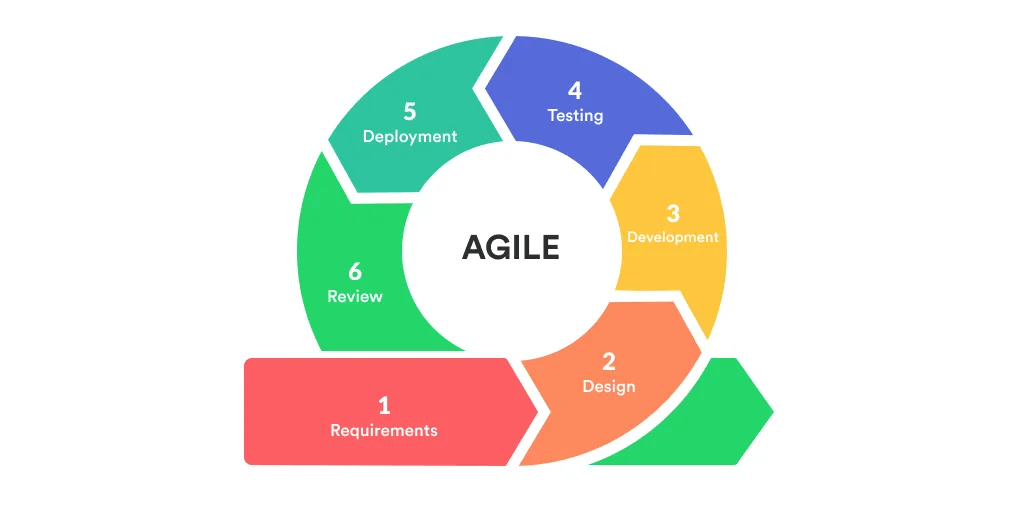
\includegraphics[width=\textwidth]{AGILE}
\end{figure}

\subsection{Planning}

	In the initial phase, the researchers outlined the shelter location allocation system's scope, objectives, and requirements. This process identifies the key features and functionalities essential for the system. Additionally, this phase includes the thesis project plan, which details the project timeline.
	The Gantt chart outlines the phases of the thesis project, including thesis one output, thesis two output, data collection and preparation, paper miscellaneous, system design, system development, and system assessment. Each phase addresses specific objectives that contribute to completing the shelter location-allocation system. The Gantt chart is shown in Figure 2.
	
	\begin{figure}[h!]
		\caption{The Gantt Chart}
		\centering
		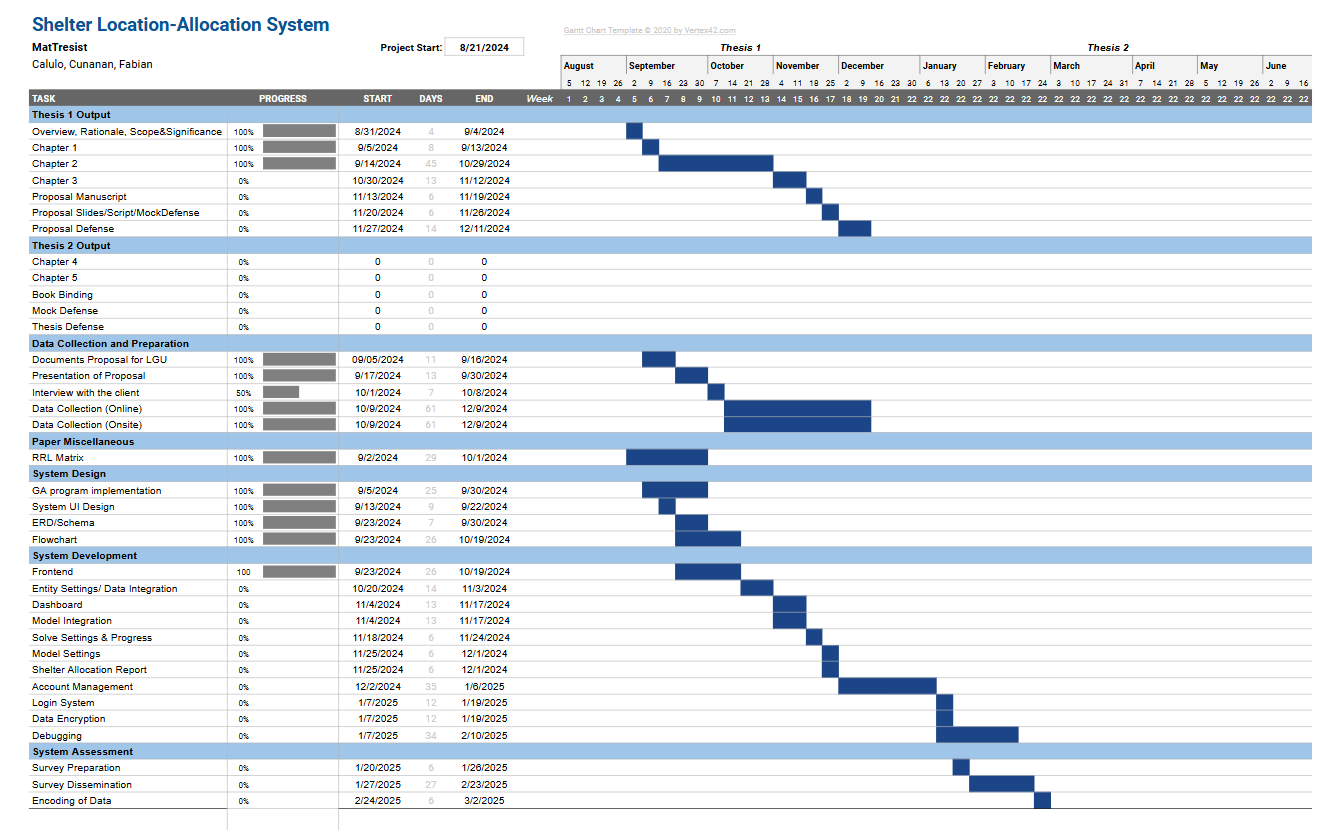
\includegraphics[width=\textwidth]{Gantt}
	\end{figure}
	
	\textbf{Thesis One Output:} This phase involves drafting the initial sections of the thesis, such as the overview, rationale, scope, and significance, along with Chapters one through three (Introduction, Review of Related Literature, and Methodology). Additionally, this phase includes preparing the proposal manuscript, slides, and script for the mock defense and proposal defense. Parallel to this is the Paper Miscellaneous, which includes the creation of the literature review matrix to organize and support the contents of Chapter 2. This approach maintains a well-structured reference base for literature review.
	
	\textbf{Thesis Two Output:} Following the foundational work in the first thesis phase, this continues the development of this thesis document, focusing on Chapters 4 and 5 (Results and Conclusions) and preparing for the mock defense and final thesis defense. This phase signifies the completion of the thesis writing process.
	
	\textbf{Data Collection and Preparation:} This critical phase entails gathering data required for system design and important data for the genetic algorithm. Tasks include submitting documents to the LGU, presenting the project proposal, conducting client interviews, and collecting online and onsite data.
	
	\textbf{System Design:} This phase focuses on planning the technical aspects of the shelter allocation system, including genetic algorithm implementation, user interface design, entity relationship diagram, and flowchart development. These elements form the blueprint that guides the system's development.
	
	\textbf{System Development:} The project's core phase involves the actual construction and coding of the system. Tasks include front-end development, data integration, model integration, dashboard creation, and implementing security features. This phase also includes testing and debugging to ensure system functionality.
	
	\textbf{System Assessment:} The final phase, along with Thesis Two Output, is evaluating the system's acceptability and user satisfaction. Activities include preparing and distributing surveys, gathering user feedback, and encoding and analyzing this data to assess system performance.

\subsection{Requirement Analysis}
	During the requirement analysis phase, researchers gather comprehensive information about the system requirements by reviewing relevant literature that pertains to the thesis. This phase ensures that all necessary features are identified and prioritized based on their importance.
	
	The system's primary features and requirements encompass an overview of data modification, data simulation, shelter tagging, and system security. Data modification includes an admin role responsible for managing community and shelter data, which can modify shelter and community data; data simulation utilizes the community and shelter data as inputs for the genetic algorithm applied in the shelter location allocation system, optimizing the placement of evacuees in shelters. Furthermore, shelter tagging enables the categorization of shelters based on criteria such as location, capacity, and suitability for various disaster scenarios, thereby facilitating efficient resource allocation. Lastly, system security ensures data protection and controlled access to maintain the integrity and confidentiality of the information managed by the system.

\subsection{Design}
	During the design phase, the researchers created a detailed design outlining the shelter location-allocation system's architecture and key components. The design process includes creating a mockup of the system's user interface and constructing flowcharts, an entity-relationship diagram (ERD), and a context diagram to map out system processes and data relationships. The researchers designed mockups to visualize the user interface, ensuring it met the user's needs for accessibility and usability. The flowcharts provided a step-by-step breakdown of system processes, while the ERD defined the data structures and relationships. These elements formed a cohesive blueprint to guide the system's development and ensure alignment with the system's requirements. The context diagram can be shown in figure 3.

	\begin{figure}[h!]
		\caption{The Context diagram}
		\centering
		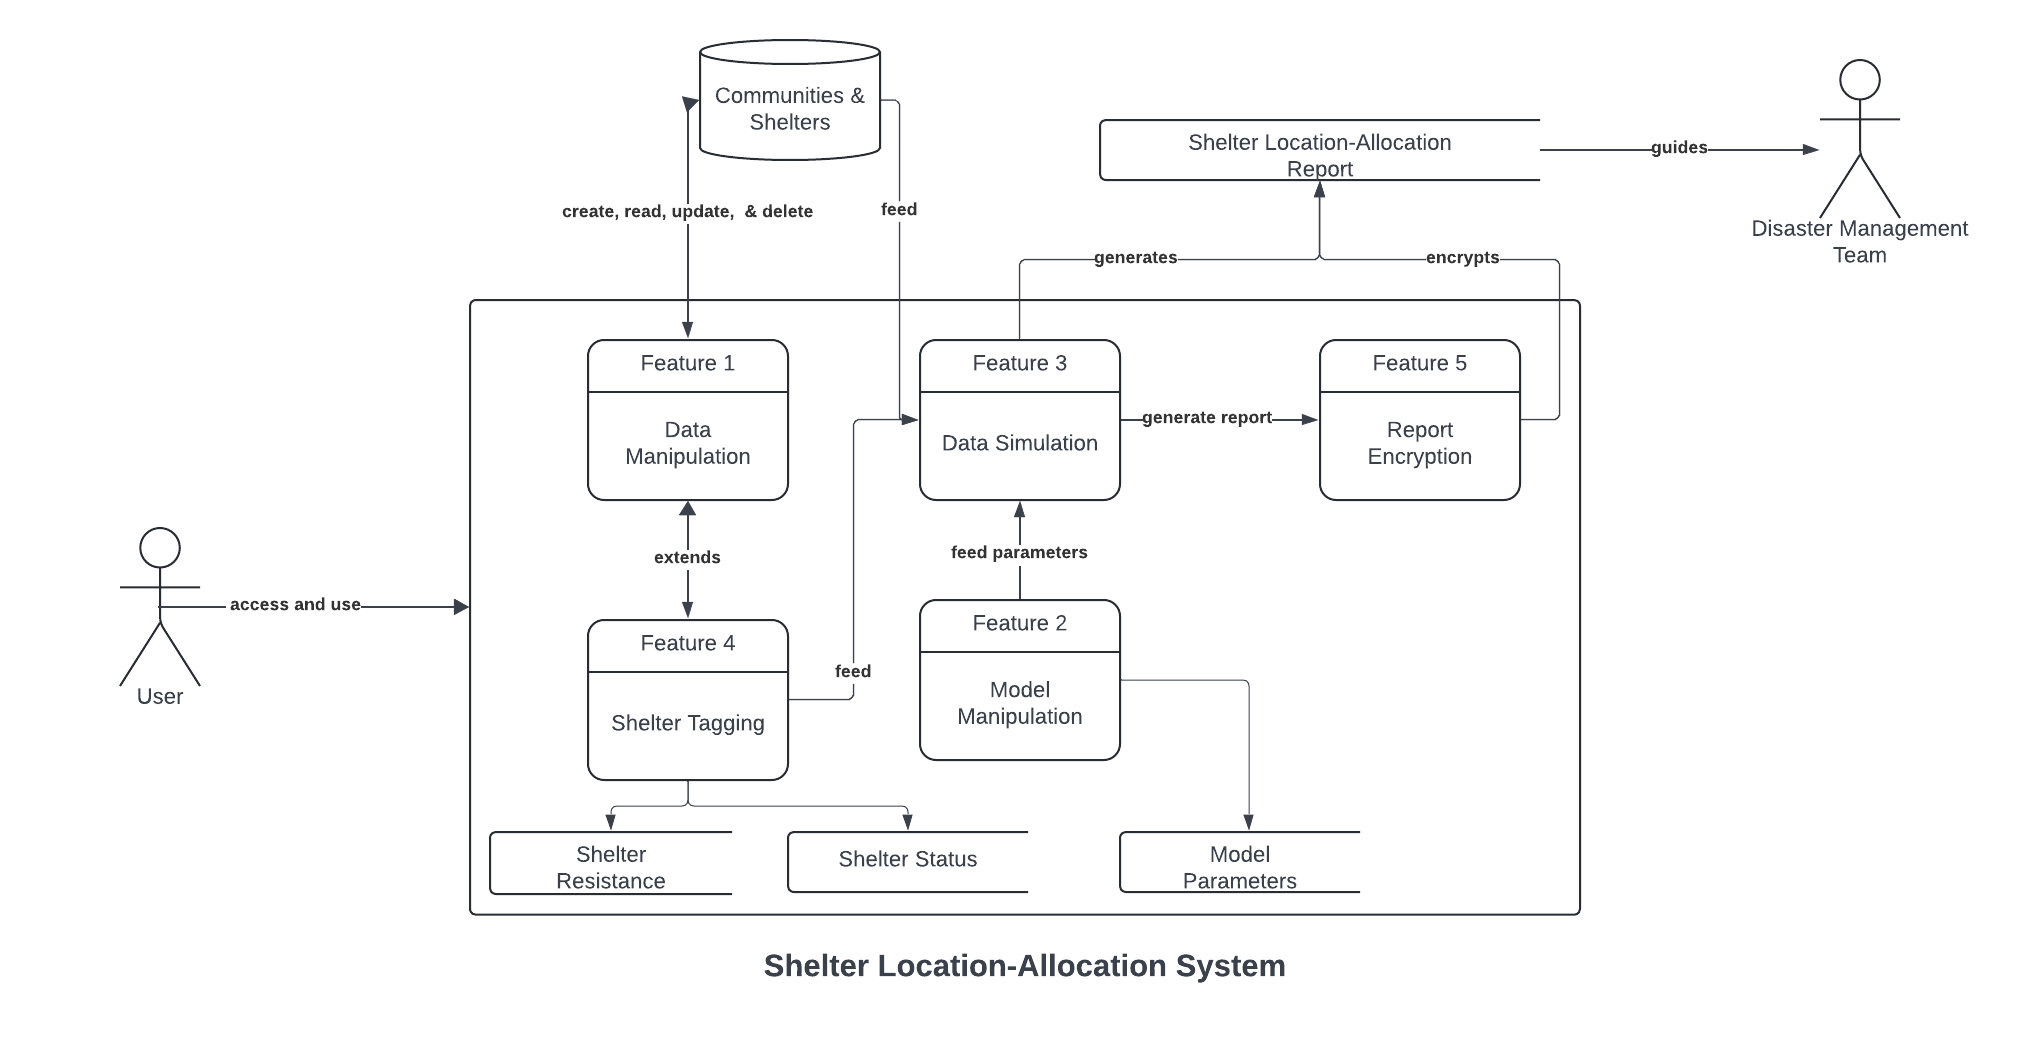
\includegraphics[width=\textwidth]{Context Diagram}
	\end{figure}
	
	The system architecture involves the interaction of two actors, the user of the system and the disaster management team. The community and shelter data will be fed into a system which features data manipulation and shelter tagging. With the cleaned or finished data, data simulation may begin together with the model parameters modified by the user. Finally, a report will be generated and can be encrypted or not. The report will be used by the disaster management team to guide them for decision making in allocation of residents to the correct shelter.

	\begin{figure}[h!]
		\caption{The ERD Schema}
		\centering
		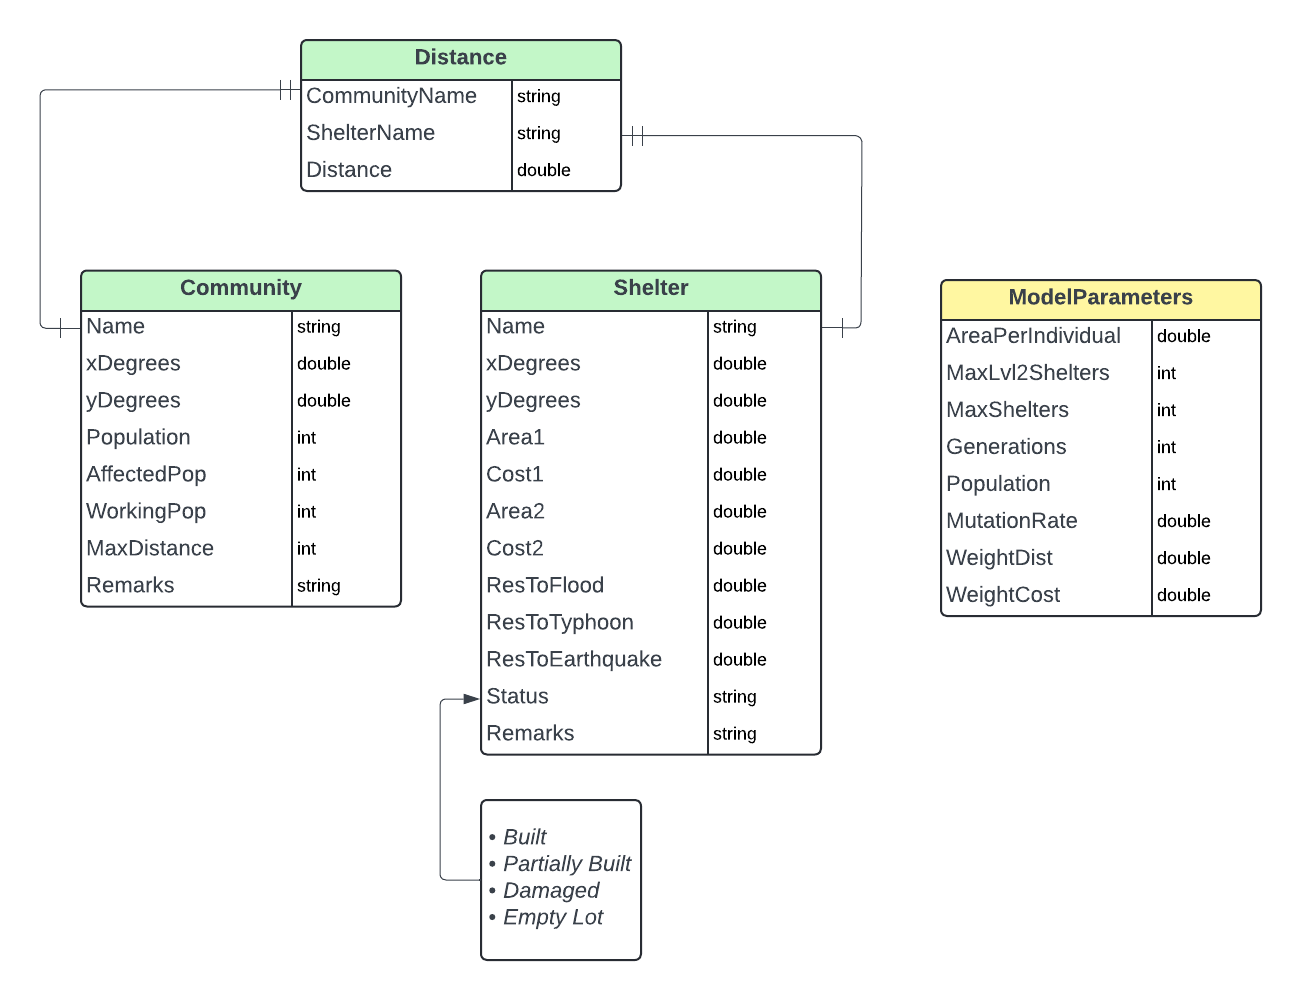
\includegraphics[width=\textwidth]{ERD}
	\end{figure}
	
	Figure 4 shows the entity relationship (ERD) which has 4 entities: Community, Shelter, Distance, and ModelParameters. Distances are derived from the location of Shelter and Community and will be saved accordingly to be used in performing the system model. ModelParameters shows no relationship since it only saves the current settings for the model and algorithm.
	
	\begin{figure}[h!]
		\caption{Examples of the system mockup}
		\centering
		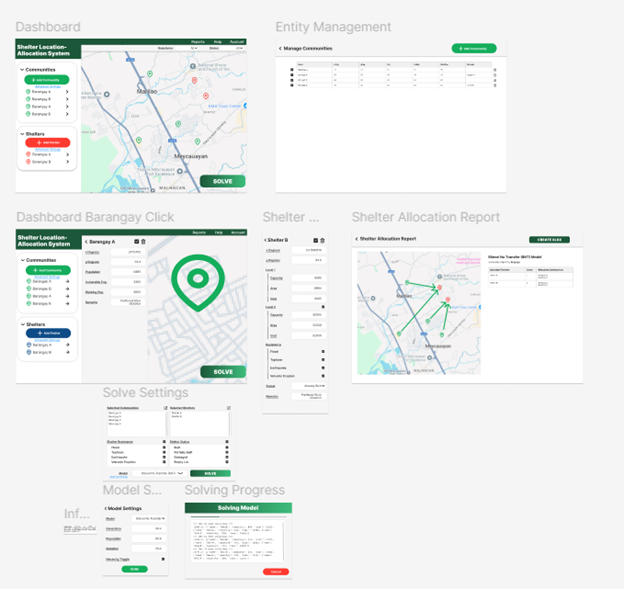
\includegraphics[width=\textwidth]{SYSTEM MOCKUP}
	\end{figure}
	
	As can be seen in Figure 5, The system mock-up shows the prototype of the system by designing the User Interface (UI) using a prototyping tool, Figma. This shows the UI for the different modules of the system: Dashboard, Entity Management, Shelter Allocation Report, Settings, and the Progress.

\subsection{Development}
	The development phase will include coding and implementing the genetic algorithm for the shelter location allocation system. Utilizing the Agile system development life cycle, which includes weekly meetings and development reviews, the team can ensure that development remains on track and that any issues are promptly addressed. By following the Agile SDLC, the researchers can adapt quickly to any changes in requirements, maintain clear communication, and address any issues promptly.
	
\subsection{Testing}
	The system will undergo functionality, performance, and reliability testing during the testing phase. The researchers will employ manual testing techniques to identify and resolve any bugs or issues that arise. This phase will also evaluate the system against the ISO/IEC 25010 standard to ensure its usability, reliability, and overall quality. Through this thorough testing approach, the researchers aim to ensure that the shelter location allocation system meets high quality, performance, and user satisfaction standards, making it ready for deployment.
	
\subsection{Deployment}
	During the deployment phase, the shelter location-allocation system will undergo pilot testing in collaboration with local government units (LGUs). This process will involve configuring the system, establishing the necessary data inputs, and training users to utilize the platform effectively. Additionally, the deployment phase will continuously monitor the system's performance to ensure it operates efficiently and meets the objective of optimizing shelter locations. 

\subsection{Maintenance}
	The maintenance phase will thoroughly identify and resolve any issues or bugs that may arise during regular operations. Maintenance involves actively monitoring the system's performance and user feedback to ensure a swift response to any problems encountered. Additionally, the researchers will prioritize implementing new features and enhancements based on valuable user feedback, ensuring the system evolves to meet user needs effectively.
	
\subsection{Evaluation}
	This section will focus on assessing the acceptability of the shelter location allocation system using the ISO/IEC 25010 standard. This standard provides a framework for evaluating the software's quality, usability, reliability, and performance efficiency. The system evaluation will include the evaluation instrument, determining the population and sample, outlining data collection procedures, and discussing the data analysis techniques used.

\section{System Evaluation}
	The evaluation instrument is a structured questionnaire designed to assess the acceptability of the shelter location allocation system based on the key quality attributes outlined in the ISO/IEC 25010 standard. The questionnaire will evaluate various aspects of the system, including usability, reliability, performance efficiency, and overall user satisfaction. Through this instrument, the study aims to gather objective data that will help determine how well the system meets user needs and expectations.

\subsection{Evaluation Instrument}
	\textbf{Functional Suitability:} This evaluates how well the system meets user needs and performs its intended functions. The questions will focus on the system's ability to allocate shelters effectively, manage community and shelter information, and provide accurate data.
	
	\textbf{Performance Efficiency:} This attribute will evaluate the system's response time and processing capacity. The questionnaire will include items assessing the system's speed in performing functions, efficient use of resources such as memory and processing power, and ability to handle maximum load requirements. By examining performance efficiency, the study aims to determine whether the system can perform reliably under diverse operational conditions.
	
	\textbf{Compatibility:} This will assess the system’s ability to exchange and use information with other systems. The questionnaire will ask how well the system integrates with external databases, applications, or systems. 
	
	\textbf{Usability:} This will prioritize the system's usability, learnability, and overall user satisfaction. The questionnaire will gather detailed user feedback regarding their experiences with the system. The questionnaire will address aspects such as ease of navigation, effectiveness in completing tasks, and general user engagement.
	
	\textbf{Reliability:} This attribute will assess the system's interaction capability, focusing on its ease of use, appropriateness for users, and ability to guide users in completing tasks effectively. The evaluation will include questions on how easily users can recognize if the system meets their needs, learn its functions, and operate it with minimal errors. Additional focus will be on user engagement, inclusivity, and the availability of assistance to support a diverse range of users. 
	
	\textbf{Security:} The system ensures that all collected data will remain confidential and solely for this research. No data will be uploaded online, and all information will be stored offline. Access to data will be limited to the researchers and users.
	
	\textbf{Maintainability:} This will evaluate the system's ease of adaptability to meet new requirements, correct errors, and improve performance. The questionnaire will assess the system's reusability, analyzing how parts of the system can be leveraged in future developments or other systems, and its testability, ensuring that any necessary changes can be efficiently implemented and quickly identified so that testing can be done efficiently. 

\subsection{Population and Sample}
	The population of this study will consist of PDRRMC, PSWDC, MDRRMC, and MSWDC of the municipality of Marilao. The diversity of the perspective of these are important for the comprehensive evaluation of the system’s acceptability.
	
	\textbf{PDRRMC:} The staff consists of Provincial Disaster Risk Reduction Management Council members of Bulacan, who are responsible for formulating and implementing the province's disaster risk reduction plan. Their input is important in aligning the shelter location allocation system.
	
	\textbf{PSWDC:} The Provincial Social Welfare and Development Council in Bulacan plays a key role in managing the evacuation and welfare of the communities during disasters. Their expertise is essential in ensuring that the shelter allocation system aligns with evacuees' specific needs, such as accessibility and capacity to the shelter location allocation across the province.
	
	\textbf{MDRRMC:} This group comprises individuals within the MDRRMC who are responsible for disaster preparedness, response, and recovery operations at the municipality of Marilao. Their insights are vital for understanding the operational requirements considerations for implementing the shelter location allocation system, ensuring it aligns with established disaster response protocols and local needs.
	
	\textbf{MSWDC:}  This group includes personnel from the MSWDC who are responsible for managing evacuees during disaster events. Their perspectives are crucial for understanding the needs and challenges involved in shelter allocation, particularly in ensuring that evacuee management is effectively integrated into the system’s functionality. Their input will help tailor the system to address the welfare requirements of evacuee management during emergencies.
	
	Since the population is small, the study will include the entire population as the sample to ensure comprehensive representation, to capture the perspectives of different stakeholder groups proportionately.

\subsection{Data Collection Procedures}
	Data collection for this project will be conducted in two main phases: the first focused on gathering data for system development, and the second on system evaluation.
	
	\textbf{For System Development:} This phase aims to establish a foundational understanding of current disaster-response processes, along with gathering essential data for the system. Interviews will be conducted with representatives from local government units (LGUs) specifically from the target population to understand their existing shelter allocation process, challenges, and expectations for a decision support system. 
	
	Additionally, to ensure that the system produces outputs, data on shelters, disaster events, and typhoons will be collected. This includes accessing records on past typhoon impacts, available shelter locations, and their respective capacities. Community or barangay data will be sourced from publicly available databases, such as PhilAtlas, which provides detailed geographical and demographic information essential for accurate system modeling.
	
	\textbf{For System Evaluation:} After system development, an evaluation phase will gauge the system’s acceptability and user satisfaction. To do this, a questionnaire will be developed based on the ISO/IEC 25010 software quality model, which will employ a 10-point Likert scale, allowing participants to provide precise feedback on each quality criterion. The system will be demonstrated to a selected sample population in a face-to-face presentation, where they will have the chance to interact with the system firsthand. This will be followed by the completion of the questionnaire, enabling participants to provide feedback based on their experience using the system.
	
	Through this structured, two-phase data collection process, the study aims to gather comprehensive and reliable information to support the development and evaluation of the shelter location allocation system. Following ISO/IEC 25010 standards ensures that the system meets its intended objectives and offers insights into potential areas for improvement, which will be critical for broader implementation in disaster-response operations. Through the data collection process, the researchers will ensure that all ethical considerations are thoroughly addressed to uphold the integrity and privacy of the participants

\subsection{Data Processing and Analysis}
	Once data collection is complete, the gathered information will undergo several stages: cleaning, processing, analysis, and interpretation. This ensures it meets the needs of the system and allows for an accurate assessment of its effectiveness.
	
	All collected data will first be cleaned to remove any inconsistencies, duplicates, or irrelevant information. This process is crucial for ensuring the data’s quality and reliability, particularly for a system that relies on precision in both inputs and outputs. Any insufficient data will be asked on the LGU to fill in the gaps of the datasets. 
	
	For justification of the target area’s vulnerability, typhoon data spanning from 2006 to 2022 will be examined. This dataset includes the number of affected and evacuated individuals across various municipalities in Bulacan. The data will be grouped by municipality, summing the affected and evacuated residents over the specified period. This analysis helps justify the focus on Bulacan and supports the rationale for the shelter allocation model’s implementation in the municipality.
	
	The cleaned shelter and community data will be fed into the system to facilitate accurate shelter location allocation modeling. The system will use these inputs to generate optimized shelter placement recommendations based on the model adopted.
	
	The structured survey, which is the second phase of data collection, will be given to the PDRRMC, PSWDC, MDRRMC, and MSWDC staff to evaluate the system's acceptability and provide critical feedback for further refinement.
	
	This study's data processing will involve structured analysis to interpret findings from the acceptability survey, aligning with the ISO/IEC 25010 standard. This standard evaluates key quality attributes, and each attribute will be assessed using a 10-point Likert scale. 1 being the lowest or extremely disagree, and 10 being the highest or extremely agree. The Table below shows the description of each numerical data.
	
	\begin{table}[h]
		\centering
		\begin{tabular}{|c|c|}
			\hline
			1  & Extremely Disagree   \\ \hline
			2  & Moderately Disagree  \\ \hline
			3  & Little more disagree \\ \hline
			4  & Mildly disagree      \\ \hline
			5  & Partially disagree   \\ \hline
			6  & Partially agree      \\ \hline
			7  & Mildly agree         \\ \hline
			8  & Little more agree    \\ \hline
			9  & Moderately agree     \\ \hline
			10 & Extremely agree      \\ \hline
		\end{tabular}
	\end{table}
	
	After the data collection and summarization, the 10-point Likert scale will categorize the acceptability levels. This dual use of data allows both the system functionality and its user acceptability to be comprehensively assessed. 

\section{Ethical Considerations}
	Data gathered contained sensitive data so that ethical considerations should be practiced throughout the research.  Informed consent will be obtained from each participant, providing them with a clear understanding of the research purpose, procedures, and their rights to withdraw at any time. To protect the participants’ privacy, all responses will be anonymized and handled with strict confidentiality. Additionally, data usage will be restricted to research purposes only, ensuring that participants' information remains safeguarded throughout the research process and beyond. 
	
	\textbf{Informed Consent:} All respondents are informed about the purpose, procedures, and potential impacts of the study before they agree to participate. The respondents will be given a detailed explanation of the study, including the nature of their involvement, the voluntary nature of participation, and their right to withdraw at any time.
	
	\textbf{Confidentiality and Anonymity:} Personal identifiers are removed from the data to ensure that the respondents cannot be traced back to other respondents. Data are stored securely, and access will be restricted to the researchers. Any publications or presentations resulting from the study will use aggregated data with no individual responses disclosed, safeguarding the identity and privacy of all respondents.
	
	\textbf{Data Protection:} The study will adhere to relevant data protection regulations, such as local data protection laws, ensuring the secure handling and storage of all collected data. Informing the respondents about how their data will be collected, stored, and used. Their rights to privacy and data protection will be respected, and only authorized researchers will have access to the information.
	
	\textbf{Minimizing Harm:} The study will be structured to minimize any potential harm to respondents. This includes ensuring that all questions are respectful, non-discriminatory, and that the data collection process does not inconvenience the respondents. Any potential risks will be clearly communicated, and measures will be implemented to mitigate these risks and uphold the respondents well-being throughout the study.
	
	\textbf{Transparency and Honesty: } The researchers will uphold transparency and honesty throughout every stage of the study. This commitment includes accurately reporting research findings, acknowledging limitations, and strictly avoiding data manipulation or bias. Respondents will be informed of the study's progress, purposes, and outcomes, ensuring they remain fully aware of how their contributions are utilized and valued within the research.
	
	By adhering to these ethical principles, the study will safeguard respondents' rights and well-being, uphold the integrity of the research process, and enhance the credibility and reliability of its findings. This ethical approach shows trust between researchers and respondents, contributing to meaningful and responsible research outcomes.
